% Created 2019-05-03 Fri 12:40
% Intended LaTeX compiler: pdflatex
\documentclass[10pt,a4paper]{article}
\usepackage[utf8]{inputenc}
\usepackage[T1]{fontenc}
\usepackage{graphicx}
\usepackage{grffile}
\usepackage{longtable}
\usepackage{wrapfig}
\usepackage{rotating}
\usepackage[normalem]{ulem}
\usepackage{amsmath}
\usepackage{textcomp}
\usepackage{amssymb}
\usepackage{capt-of}
\usepackage{hyperref}
\usepackage[margin=2cm]{geometry}
\author{Mikael Svahnberg\thanks{Mikael.Svahnberg@bth.se}}
\date{\today}
\title{Example: Robot System}
\hypersetup{
 pdfauthor={Mikael Svahnberg},
 pdftitle={Example: Robot System},
 pdfkeywords={},
 pdfsubject={},
 pdfcreator={Emacs 25.3.1 (Org mode 9.1.2)}, 
 pdflang={English}}
\begin{document}

\maketitle
\tableofcontents


\section{Introduktion}
\label{sec:orgbdc108a}
Det här är ett exempel som vi började arbeta med på lektionen den \textit{<2019-05-03 Fri>}, med tanke att fortsätta nästa lektion. Exemplet är inte komplett och förmodligen svårt att hänga med på om man inte var med på föreläsningen; om du är osäker så fråga dina studentkollegor.
\section{Package Diagram}
\label{sec:org11d7a63}
\begin{verbatim}
package UI

package Robot {
package ControlInterface
package Navigation
package Steering
package ArmControl

ControlInterface - Navigation
ControlInterface - Steering

}

package HardwareControllers {
package Motors
package Sensors
}

UI - Robot
Steering - Motors
Navigation - Sensors
ArmControl - Motors
ArmControl - Sensors

\end{verbatim}

\begin{center}
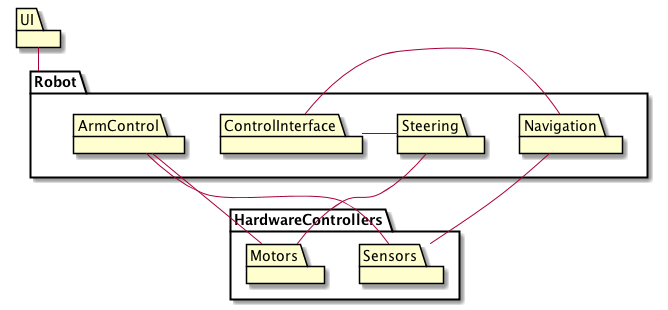
\includegraphics[width=.9\linewidth]{packdia.jpg}
\end{center}

\section{Use Case: Navigate to Point}
\label{sec:orgd6f0d3e}
\textbf{Use Case}: Navigate to Point

\textbf{Actors}: User

\textbf{Description}: User selects a coordinate and asks for routes to this point. System displays possible routes. User selects one route. 

\textbf{Requirements:} FR120, QA2, FR111

\textbf{Main Course of Events}
\begin{center}
\begin{tabular}{ll}
Actor & System\\
\hline
1. User selects ``Navigate to Point'' & \\
 & 2. System displays a map and asks user to select a point\\
3. User selects a point & \\
 & 4. System calculates routes and displays them.\\
5. User selects one route. & \\
\hline
\end{tabular}
\end{center}

\section{Systemsekvensdiagram: Navigate to Point}
\label{sec:org6a6efe9}
\begin{verbatim}
actor user
participant ":system" as sys

user -> sys : selectNavigationMethod("toPoint")
sys --> user : displays map, asks for a destination

user -> sys : selectPoint(x,y)
sys --> user : displays alternative rotues

user -> sys : selectNearestRoute(x,y)
sys --> user : confirms rute

\end{verbatim}

\begin{center}
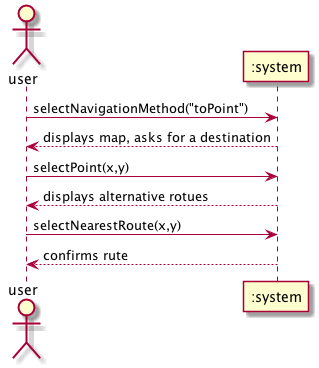
\includegraphics[width=.9\linewidth]{robot-ssd.png}
\end{center}

\section{Sekvensdiagram - selectNavigationMethod}
\label{sec:org4dcb6dd}
\begin{verbatim}
[-> ":system" : selectNavigationMethod("toPoint")
activate ":system"

create "currentNavigationStrategy:PointNavigation" as cns
":system" -> cns : create()
activate cns
cns -> ":GPS" : currentCoordinates = getCurrentCoordinates()
activate ":GPS"
deactivate ":GPS"

cns -> ":MapCollection" : getMap(currentCoordinates, zoomLevel)
activate ":MapCollection"
create "map:Map"
":MapCollection" -> "map:Map" : create()
":MapCollection" --> cns : map:Map
deactivate ":MapCollection"
deactivate cns

":system" -> cns : getResponseObject()
activate cns
create "response:ResponseObject"
cns -> "response:ResponseObject" : create()

alt map exists
cns -> "response:ResponseObject" : setMap(map)
else
cns -> "response:ResponseObject" : setError("Map does not exist")
end

cns --> ":system" : return responseObject
deactivate cns

":system" -->[ : map around current location

deactivate ":system"

\end{verbatim}

\begin{center}
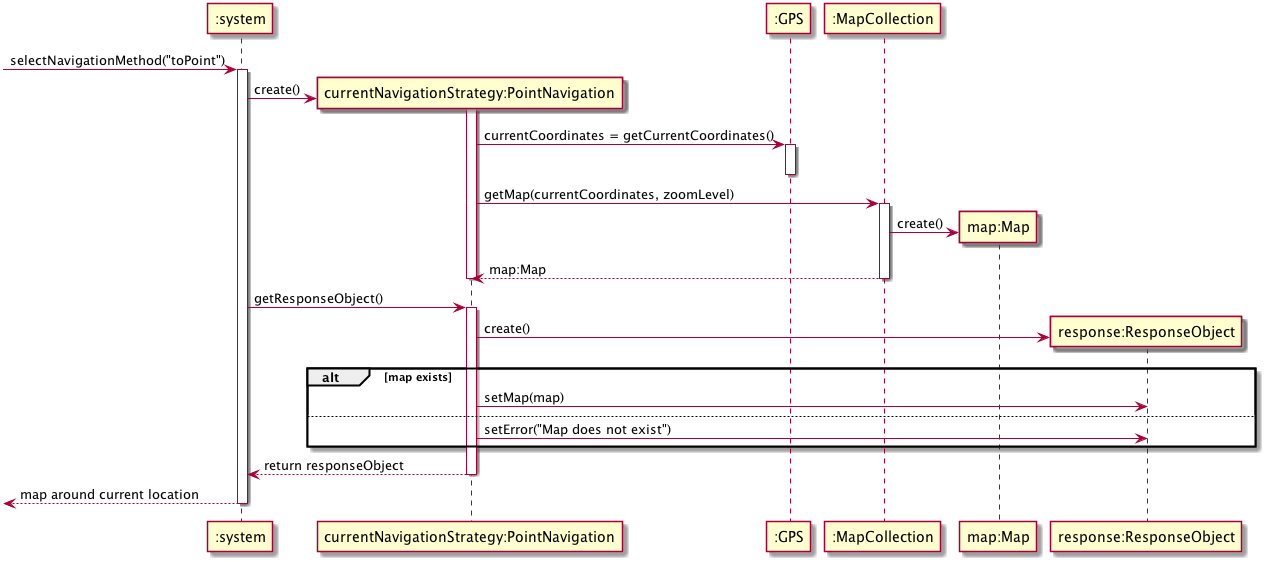
\includegraphics[width=.9\linewidth]{robot-selectnavigationmethod.png}
\end{center}

\section{Klassdiagram}
\label{sec:org5b5f210}
Såhär ser t.ex. metoden selectNavigationMethod i klassen system:
\begin{verbatim}
system::selectNavigationMethod(String theMethod) {
// ...
NavigationMethod* currentNavigationMethod = new PointNavigation(); // create()
// ...
ResponseObject* ro = currentNavigationMethod->getResponse();
// ...
return ro;
}
\end{verbatim}

Klassdiagram med alla klasser, metoder, och relationer från sekvensdiagrammet för systemhändelsen selectNavigationMethod():
\begin{verbatim}
class system {
+selectNavigationMethod(theMethod)
}
class PointNavigation {
+create()
+getResponse()
- currentPosition:Position
- map : Map
}
class GPS {
+ getCurrentCoordinates()
}
class MapCollection {
+ getMap(coordinates, zoomLevel)
}
class Map {
+create()
}
class ResponseObject {
+setMap(theMap:Map)
+setError(string theError)
}

system - NavigationMethod
NavigationMethod <|-- PointNavigation
system -- ResponseObject
PointNavigation -- GPS
PointNavigation -- MapCollection
PointNavigation -- Map
PointNavigation -- ResponseObject
MapCollection - Map
ResponseObject - Map

\end{verbatim}

\begin{center}
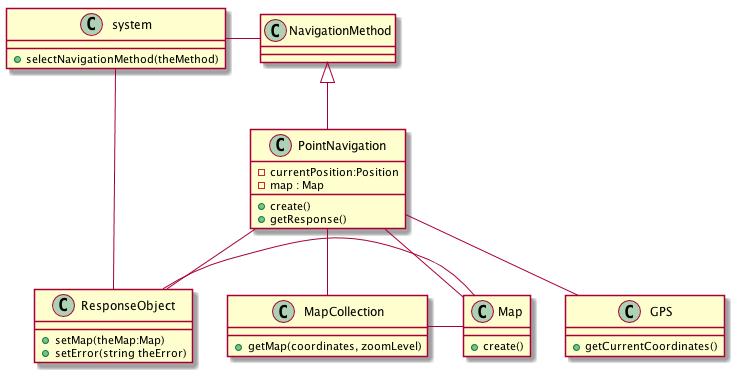
\includegraphics[width=.9\linewidth]{robot-class.png}
\end{center}
\end{document}